\documentclass[10pt,pdf,hyperref={unicode}]{beamer}

\mode<presentation>
{
	\usetheme{boxes}
	\beamertemplatenavigationsymbolsempty
	
	\setbeamertemplate{footline}[page number]
	\setbeamersize{text margin left=0.5em, text margin right=0.5em}
}

\usepackage[utf8]{inputenc}
\usepackage[english, russian]{babel}
\usepackage{bm}
\usepackage{multirow}
\usepackage{ragged2e}
\usepackage{indentfirst}
\usepackage{multicol}
\usepackage{subfig}
\usepackage{amsmath,amssymb}
\usepackage{enumerate}
\usepackage{mathtools}
\usepackage{comment}
\usepackage{multicol}

\usepackage[all]{xy}

\usepackage{tikz}
\usetikzlibrary{positioning,arrows}

\tikzstyle{name} = [parameters]
\definecolor{name}{rgb}{0.5,0.5,0.5}

\usepackage{caption}
\captionsetup{skip=0pt,belowskip=0pt}

\newtheorem{rustheorem}{Теорема}
\newtheorem{russtatement}{Утверждение}
\newtheorem{rusdefinition}{Определение}

% colors
\definecolor{darkgreen}{rgb}{0.0, 0.2, 0.13}
\definecolor{darkcyan}{rgb}{0.0, 0.55, 0.55}

\AtBeginEnvironment{figure}{\setcounter{subfigure}{0}}

\captionsetup[subfloat]{labelformat=empty}

%----------------------------------------------------------------------------------------------------------

\title[Метод построения случайного леса на основе отдаления друг от друга базовых моделей]{Метод построения случайного леса на основе отдаления друг от друга базовых моделей}
\author{Дмитриев\,Леонид\,Алексеевич\\Сенько\,Олег\,Валентинович}

\institute[]{Московский государственный университет им. М. В. Ломоносова}
\date[2023]{\small 15\;февраля\;2023\,г.}

%---------------------------------------------------------------------------------------------------------
\begin{document}
	
	\begin{frame}
		\titlepage
	\end{frame}
	
	%----------------------------------------------------------------------------------------------------------
	\section{Введение}
	\begin{frame}{Введение}
		\bigskip
		Случайный лес - широко известный алгоритм машинного обучения. Его способность хорошо аппроксимировать данные за счёт уменьшения разброса основана на предположении, что все деревья ансамбля независимы и различны.\\
		\bigskip
		\textbf{Проблема}: практическое уменьшение разброса значительно меньше теоретического, так как на деле получаемые деревья обучаются на объектах из одного и того же множества.\\
		\bigskip
		\textbf{Цель работы}: предложить другой способ повышения разнообразия деревьев внутри леса и показать его применимость.\\
		\bigskip
		\textbf{Идея}: вместо независимой и параллельной генерации деревьев, будем на каждом шагу добавлять дерево, сильно отличающееся от уже созданного ансамбля, с помощью специального функционала, учитывающего ответы предыдущих моделей.
	\end{frame}
	
	%---------------------------------------------------------------------------------------------------------
	\section{Постановка задачи}
	\begin{frame}{Постановка задачи}
		
		Имеется выборка $\tilde{S} = \{ (y_j, x_j, G_1(x_j), G_2(x_j)), j = \overline{1, m} \}$, где
		\begin{itemize}
			\item $y_j$ - значение переменной $Y$ для объекта с номером $j$
			\item $x_j = (x_{j1}, \dots, x_{jn})$ - вектор значений признаков $X_1, \dots, X_n$ для объекта с номером $j$
			\item $G_1(x_j)$ - значение функции $G_1$ в точке $x_j$
			\item $G_2(x_j)$ - значение функции $G_2$ в точке $x_j$
		\end{itemize}
		
		Предлагается построить дерево $T(x)$, для которого достигается минимум функционала:
		$$ \Phi(\tilde{S}, T) = \Sigma_{j=1}^{m} \{ \gamma_1 [T(x_j) - y_j]^2 + \gamma_2 [T(x_j) - G_2(x_j)]^2 - \mu [T(x_j) - G_1(x_j)]^2   \}  $$
		где $\gamma_1 + \gamma_2 = 1; \quad \gamma_1, \gamma_2, \mu \in [0, 1] $
		
		\bigskip
		
		Вместо независимой и параллельной генерации деревьев,
		будем на каждом шагу добавлять дерево, сильно отличающееся от уже
		созданного ансамбля, с помощью специального функционала,
		учитывающего ответы предыдущих моделей.
		

	\end{frame}
	

	%----------------------------------------------------------------------------------------------------------
	\section{Реализация}
	\begin{frame}{Реализация}
	
	При построении дерева был использован "жадный" \space метод оптимизации целевого функционала: на каждом шагу к дереву добавляется узел, обеспечивающий наибольшее снижение используемого функционала $\Phi$.

	Предположим, что на каком-то шаге дерево $T_k$ содержит $k$ концевых узлов, которым соответствуют концевые выборки $S_1^k, \dots, S_k^k$.

	Новое дерево $T_{k + 1}$ строится через добавление к дереву $T_k$ дополнительного узла $u$.

	Узел $u$ получается из некоторого концевого узла $g$ с помощью порогового правила вида $X_u > \delta_u$, где $X_u$ и $\delta_u$ признак и порог к нему соответственно. 

	Правило $X_u > \delta_u$ расщепляет выборку $S_g^k$ на две подвыборки.

	Признак $X_u$ и порог $\delta_u$ ищутся из условия максимизации разности $\Phi(\tilde{S}, T_k) - \Phi(\tilde{S}, T_{k + 1})$.

	Процесс построения может быть прекращен при выполнении одного из перечисленных условий:

	\begin{itemize}
		\item На очередном шаге не удается уменьшить функционал
		\item На очередном шаге произошло изменение функционала, меньшее чем некоторое пороговое значение
		\item Кол-во объектов внутри узла меньше некоторого порогового значения
	\end{itemize}
	
	\end{frame}
	
	%----------------------------------------------------------------------------------------------------------
	\section{Слайд об исследованиях}
	\begin{frame}{Слайд об исследованиях}
		
		\begin{figure}[h]
	\begin{center}
		\begin{minipage}[h]{0.5\linewidth}
			{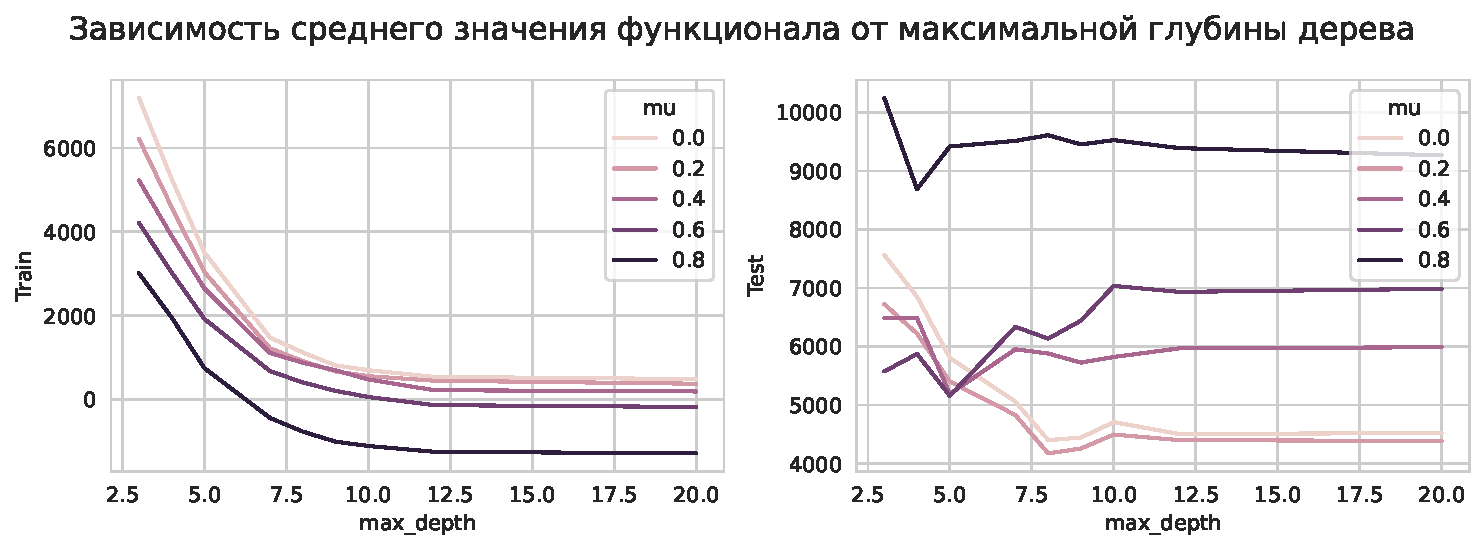
\includegraphics[width=\linewidth]{../figures/max_depth_task1_gamma_08_min_2.pdf}}	
		\end{minipage}
		\begin{center}
		\begin{minipage}[h]{0.5\linewidth}
			{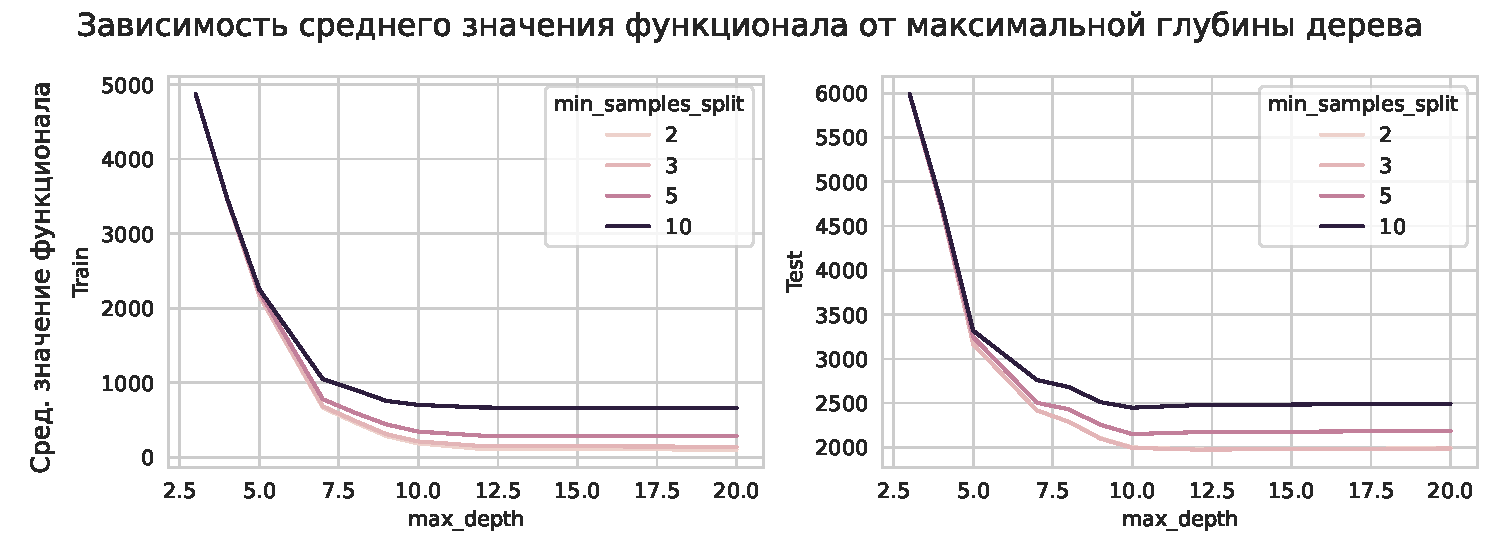
\includegraphics[width=\linewidth]{../figures/max_depth_task1_gamma_02_mu_02.pdf}}	
		\end{minipage}
	\end{center}
	\end{center}
	
	Были проведены эксперименты примения метода для задачи регрессии. Для тестирования и исследования в качестве модели G1 (к зависимости которой дерево должно приближаться) был взят градиентный бустинг, а в качестве модели G2 (от зависимости которой необходимо удаляться) случайный лес. Параметры данных моделей были подобраны на кросс-валидации, где использовалась стандартная метрика MSE. Был произведен ряд экспериментов с различными значениями гиперпараметров модели.
	
	\label{ris:image7}
\end{figure}
		
	\end{frame}
	
	%----------------------------------------------------------------------------------------------------------
	\section{Выводы}
	\begin{frame}{Выводы}
	
	В данной работе исследовался метод построения дерева с помощью специального функционала, позволяющего отдаляться от уже построенного ансамбля, с целью повышения разнообразия итогового леса. Исследование производилось на данных о химических соединениях, где целевой переменной была выбрана температура плавления.
Были проведены эксперименты, показавшие корректность реализованной модели, выявившие некоторые отличия от стандартного функционала и показавшие применимость метода.

	\end{frame}
	

	
\end{document} 